\documentclass[tikz,border=1mm]{standalone}
\usepackage{amssymb}
\usetikzlibrary{matrix,chains,positioning,decorations.pathreplacing,arrows,shapes.geometric}

% Code modified from here https://tex.stackexchange.com/questions/505741/architecture-neural-network-with-weights

\begin{document}
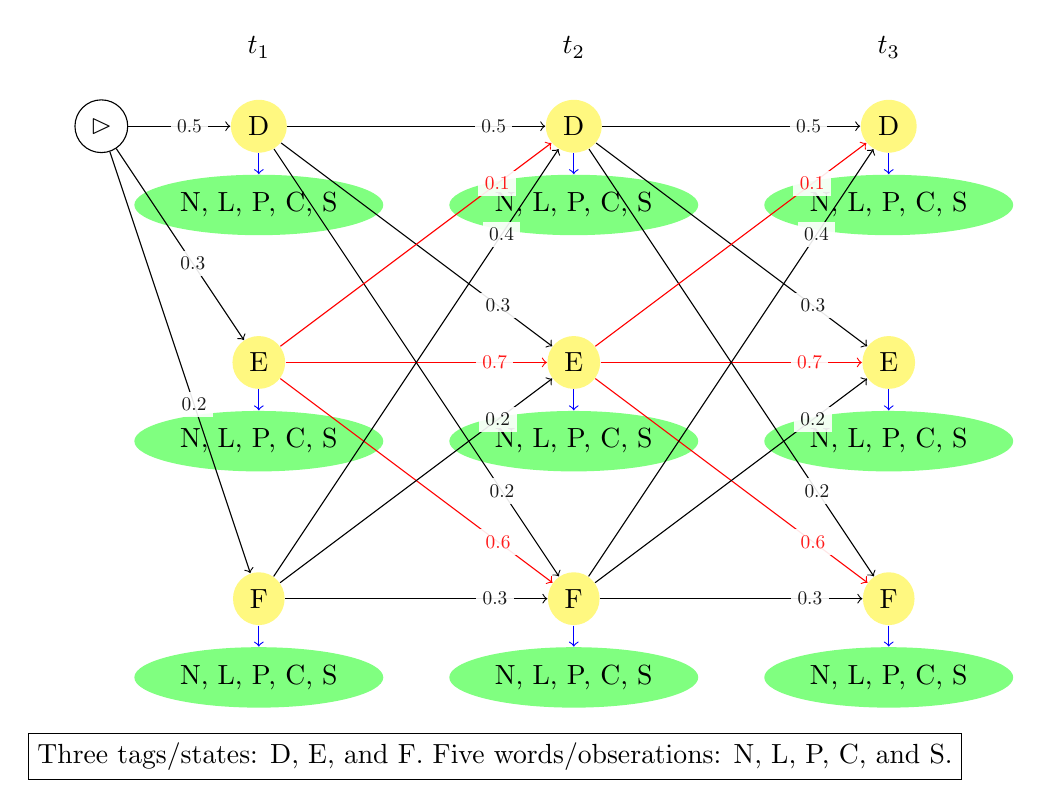
\begin{tikzpicture}%[>=latex]

% Step 1 
\path
(0,0)         node[circle,draw,align=center] (origin) {$\rhd$} 
+(2,1)     node  (t1) {$t_1$}
+(2,0)     node[ellipse,fill=yellow!50]  (t11) {D} % {$t_{1,1}$}
+(2,-1)     node[ellipse,fill=green!50]  (w11) {N, L, P, C, S}
+(2,-3)     node[ellipse,fill=yellow!50]  (t12) {E} % {$t_{1,2}$}
+(2,-4)     node[ellipse,fill=green!50]  (w12) {N, L, P, C, S}
+(2,-6)     node[ellipse,fill=yellow!50]  (t13) {F} % {$t_{1,3}$}
+(2,-7)     node[ellipse,fill=green!50]  (w13) {N, L, P, C, S}
;

\draw[->, black] (origin)--(t11) node[pos=.6, fill=white, opacity=.9, scale=0.7]{$0.5$};
\draw[->, black] (origin)--(t12) node[pos=.6, fill=white, opacity=.9, scale=0.7]{$0.3$};
\draw[->, black] (origin)--(t13) node[pos=.6, fill=white, opacity=.9, scale=0.7]{$0.2$};
\draw[->, blue] (t11)--(w11) ;
\draw[->, blue] (t12)--(w12) ;
\draw[->, blue] (t13)--(w13) ;
% End step 1 



% Step 2 
\path 
+(6,1)     node  (t2) {$t_2$}
+(6,0)     node[ellipse,fill=yellow!50]  (t21) {D} %{$t_{2,1}$}
+(6,-1)       node[ellipse,fill=green!50]  (w21) {N, L, P, C, S}
+(6,-3)     node[ellipse,fill=yellow!50]  (t22) {E} % {$t_{2,2}$}
+(6,-4)       node[ellipse,fill=green!50]  (w22) {N, L, P, C, S}
+(6,-6)     node[ellipse,fill=yellow!50]  (t23) {F} % {$t_{2,3}$}
+(6,-7)       node[ellipse,fill=green!50]  (w23) {N, L, P, C, S}
;

\draw[->, black] (t11)--(t21) node[pos=.8, fill=white, opacity=.9, scale=0.7]{$0.5$};
\draw[->, black] (t11)--(t22) node[pos=.8, fill=white, opacity=.9, scale=0.7]{$0.3$};
\draw[->, black] (t11)--(t23) node[pos=.8, fill=white, opacity=.9, scale=0.7]{$0.2$};

\draw[->, red] (t12)--(t21) node[pos=.8, fill=white, opacity=.9, scale=0.7]{$0.1$};
\draw[->, red] (t12)--(t22) node[pos=.8, fill=white, opacity=.9, scale=0.7]{$0.7$};
\draw[->, red] (t12)--(t23) node[pos=.8, fill=white, opacity=.9, scale=0.7]{$0.6$};

\draw[->, black] (t13)--(t21) node[pos=.8, fill=white, opacity=.9, scale=0.7]{$0.4$};
\draw[->, black] (t13)--(t22) node[pos=.8, fill=white, opacity=.9, scale=0.7]{$0.2$};
\draw[->, black] (t13)--(t23) node[pos=.8, fill=white, opacity=.9, scale=0.7]{$0.3$};

\draw[->, blue] (t21)--(w21) ;
\draw[->, blue] (t22)--(w22) ;
\draw[->, blue] (t23)--(w23) ;

% step 3: 
\path 
+(10,1)     node  (t3) {$t_3$}
+(10,0)     node[ellipse,fill=yellow!50]  (t31) {D}% {$t_{3,1}$}
+(10,-1)       node[ellipse,fill=green!50]  (w31) {N, L, P, C, S}
+(10,-3)     node[ellipse,fill=yellow!50]  (t32) {E}% {$t_{3,2}$}
+(10,-4)       node[ellipse,fill=green!50]  (w32)  {N, L, P, C, S}
+(10,-6)     node[ellipse,fill=yellow!50]  (t33) {F} %  {$t_{3,3}$}
+(10,-7)       node[ellipse,fill=green!50]  (w33) {N, L, P, C, S}
;

\draw[->, black] (t21)--(t31) node[pos=.8, fill=white, opacity=.9, scale=0.7]{$0.5$};
\draw[->, black] (t21)--(t32) node[pos=.8, fill=white, opacity=.9, scale=0.7]{$0.3$};
\draw[->, black] (t21)--(t33) node[pos=.8, fill=white, opacity=.9, scale=0.7]{$0.2$};

\draw[->, red] (t22)--(t31) node[pos=.8, fill=white, opacity=.9, scale=0.7]{$0.1$};
\draw[->, red] (t22)--(t32) node[pos=.8, fill=white, opacity=.9, scale=0.7]{$0.7$};
\draw[->, red] (t22)--(t33) node[pos=.8, fill=white, opacity=.9, scale=0.7]{$0.6$};

\draw[->, black] (t23)--(t31) node[pos=.8, fill=white, opacity=.9, scale=0.7]{$0.4$};
\draw[->, black] (t23)--(t32) node[pos=.8, fill=white, opacity=.9, scale=0.7]{$0.2$};
\draw[->, black] (t23)--(t33) node[pos=.8, fill=white, opacity=.9, scale=0.7]{$0.3$};

\draw[->, blue] (t31)--(w31) ;
\draw[->, blue] (t32)--(w32) ;
\draw[->, blue] (t33)--(w33) ;

\node[draw] at (5,-8) {Three tags/states: D, E, and F. Five words/obserations: N, L, P, C, and S.};

\end{tikzpicture}
\end{document}
